% [Overleaf] https://www.overleaf.com/read/nhwshxmhbrqy
% [YouTube] https://youtu.be/s4X_JroR9sE
% [GitHub] https://github.com/nobucshirai/infona2020_slide_04
\documentclass[dvipdfmx,aspectratio=169,20pt]{beamer}
\usepackage{bxdpx-beamer}

% Beamer theme
\usetheme{Boadilla}

%%%%% JAPANESE FONT SETTINGS %%%%%
\usepackage[utf8]{inputenc}
\usepackage{pxjahyper}
\renewcommand{\kanjifamilydefault}{\gtdefault} % for Gothic Japanese fonts
\newcommand{\myfontsetting}[3]{{\fontsize{#1}{#2}\selectfont #3}}
\usepackage[deluxe,uplatex]{otf} % needed to use super bold Japanese fonts
\usepackage[unicode,noto-otc]{pxchfon} % needed to use super bold Japanese fonts
%%%%%%%%%%%%%%%%%%%%%%%%%%%%%%%%%%

%%%%% SETTINGS FOR MATH SYMBOLS %%%%%
\usepackage{amsmath,amssymb}
\usepackage{bm}
%\usepackage{graphicx}
\usepackage{latexsym}
\usefonttheme{professionalfonts} % use Serif fonts for equations
%%%%%%%%%%%%%%%%%%%%%%%%%%%%%%%%%%%%%

\usepackage{fancybox,ascmac}
\usepackage{url}
\usepackage[many]{tcolorbox}

%%%%% ALGORITHM SETTING %%%%%
\usepackage{algorithm}
\usepackage[noend]{algorithmic}
\algsetup{linenosize=\color{fg!50}\fontsize{8pt}{8pt}\selectfont}
\renewcommand\algorithmicdo{\bfseries :}
\renewcommand\algorithmicthen{\bfseries :}
\renewcommand\algorithmicrequire{\textbf{Input:}}
\renewcommand\algorithmicensure{\textbf{Output:}}
\renewcommand{\algorithmicprint}{\textbf{break}}
%%%%%%%%%%%%%%%%%%%%%%%%%%%%%
\definecolor{myblue1}{RGB}{45,130,200}
\definecolor{myblue2}{RGB}{26,89,142}
\setbeamertemplate{navigation symbols}{}
\setbeamercolor*{structure}{fg=myblue1,bg=blue}
\setbeamercolor{block title}{fg=myblue1!50!black}
\setbeamercolor*{block title example}{fg=white,bg=myblue2}
\setbeamercolor*{palette primary}{use=structure,fg=white,bg=structure.fg}
\setbeamercolor*{palette secondary}{use=structure,fg=white,bg=structure.fg!75!black}
\setbeamercolor*{palette tertiary}{use=structure,fg=white,bg=structure.fg!50!black}
\setbeamercolor*{palette quaternary}{fg=black,bg=myblue1}

\setbeamerfont{alerted text}{series=\bfseries}
\setbeamerfont{section in toc}{series=\mdseries}
\setbeamerfont{frametitle}{size=\Large,series=\bfseries}
\setbeamerfont{title}{size=\LARGE,series=\bfseries}
\setbeamerfont{date}{size=\small}

\setbeamertemplate{block title}[shadow=false]
\setbeamertemplate{blocks}[rounded][shadow=false]

%%%%% BEAMER FOOTLINE SETTINGS %%%%%%
\setbeamertemplate{footline}[frame number]{}
\setbeamerfont{footline}{size=\bf\footnotesize\small}
%%%%%%%%%%%%%%%%%%%%%%%%%%%%%%%%%%%%%

%%%%% BEAMER ITEM SETTINGS %%%%%
\setbeamertemplate{itemize item}[circle]
\setbeamertemplate{itemize subitem}[triangle]
\setbeamertemplate{enumerate item}[circle]
%%%%%%%%%%%%%%%%%%%%%%%%%%%%%%%%

\begin{document}

\graphicspath{{figs/}}

%%%%%%%%%%%%%%%%%%%%%%%%%%%%%%%%
\begin{frame}
%%%%% START_TAG B %%%%%
%\noindent{\bf I\hspace{-.1em}I\hspace{-.1em}I-B.}
\frametitle{[問題] I\hspace{-.1em}I\hspace{-.1em}I-B (1)}
\myfontsetting{18pt}{20pt}{
$f(x)=2-e^{x}$ が与えられた時、$x\in [0,1]$ の範囲にある $f(x)$ の根を2分法を用いて求める場合を考える。解の存在する範囲を $10^{-8}$ 以下に限定するには2分法の繰り返し操作を最低何回行えば良いか答えよ。%\\
}
\end{frame}
%%%%%%%%%%%%%%%%%%%%%%%%%%%%%%%%
\begin{frame}
\frametitle{[問題] I\hspace{-.1em}I\hspace{-.1em}I-B (2)}
\myfontsetting{18pt}{20pt}{
2分法により $f(x)$ の根を求めるプログラムを作成して問1で求めた回数繰り返し、繰り返し操作後の解の存在する $x$ の区間の両端の値を有効数字10進11桁以降を切り捨てて求めよ。またその区間の両端の値の平均値を求め根の近似値として有効数字10進11桁以降を切り捨てて求めよ。
}\\
\myfontsetting{12pt}{14pt}{
作成したプログラムも提出すること。プログラミング言語は問わない。
}
%%%%% END_TAG B %%%%%
\end{frame}
%%%%%%%%%%%%%%%%%%%%%%%%%%%%%%%%
\begin{frame}
\frametitle{[略解] I\hspace{-.1em}I\hspace{-.1em}I-B (1)}
\vspace{-0.5cm}
\begin{eqnarray*}
    &&\inf \left\{n\in \mathbb{N}\  \middle| \ \frac{1}{2^n}\le 10^{-8} \right\}\\
    &=& \inf \left\{n\in \mathbb{N}\  \middle| \ n \ge 8\log_2 10 \right\}\\
    &=& \lceil 8\log_2 10 \rceil= 27
\end{eqnarray*}
従って27回。
\end{frame}
%%%%%%%%%%%%%%%%%%%%%%%%%%%%%%%%
\begin{frame}
\frametitle{[略解] I\hspace{-.1em}I\hspace{-.1em}I-B (2)}
\vspace{-0.5cm}
解の存在する区間幅

[0.6931471750, 0.6931471824]

\vspace{0.5cm}
根の近似値 0.6931471787

\end{frame}
%%%%%%%%%%%%%%%%%%%%%%%%%%%%%%%%
%タイトルページ

\title{求根アルゴリズム (2)}
\titlegraphic{\vspace{-7mm}\flushright
\includegraphics[width=1.8cm,height=1.8cm]{hattari_kun_good_org.eps}}

\setbeamertemplate{title page}{%
    \begin{flushright}
        \usebeamercolor[fg]{titlegraphic}\inserttitlegraphic
    \end{flushright}
    \vspace{-0.6cm}
    \hspace{1.5cm}{\selectfont\usebeamerfont{subtitle} \usebeamercolor[fg]{subtitle} [\href{https://youtu.be/s4X_JroR9sE}{数値解析 第4回}] \par}
    \vspace{0.5cm}
    %\vspace{2.5em}
    {\centering\usebeamerfont{title} \usebeamercolor[fg]{title} \inserttitle \par}
    \vspace{0.5cm}
    \begin{center}
        式の根っこを速く旨く求める
    \end{center}
}

\date[\todey]{}

\frame{\titlepage}

%%%%%%%%%%%%%%%%%%%%%%%%%%%%%%%%
\begin{frame}
\frametitle{反復法}
\begin{block}{{\bf 反復法} {\small (Iterative method)}}
{\small 
式 $f(x)$ の1つの根が $\alpha$ としたとき、初期近似根 $x_0$ を与え反復式 $x_{k+1} = \varphi(x_k)$ $(k=0,1,\dots)$ によって近似根 $x_k$ を $\alpha$ に近づけて行く求根法を{\bf 反復法}という。}
\end{block}
\begin{itemize}
    %\setlength{\itemsep}{0.5cm}
    \item \myfontsetting{14pt}{16pt}{ニュートン法は $\varphi(x)=x - f(x)/f^\prime(x)$ とおいた場合の反復法}
     \item 
    \myfontsetting{14pt}{16pt}{反復法が縮小写像になっていれば不動点としての根 $\alpha$ に収束する}
\end{itemize}
\end{frame}
%%%%%%%%%%%%%%%%%%%%%%%%%%%%%%%%
\begin{frame}
\frametitle{\large 反復法で根を求めるための条件}
\begin{block}{{\bf 縮小写像} {\small (Contraction mapping)}}
\myfontsetting{14pt}{16pt}{ある区間 $I\subset \mathbb{R}$ の任意の $x$, $y$ に対して $\varphi(x)$ が $|\varphi(x)-\varphi(y)|\le L|x-y|$ を満たし、$0\le L < 1$ であるとき $\varphi(x)$ は区間 $I$ において{\bf 縮小写像}であるという。$L$ を{\bf 縮小率} という。}
\end{block}
\begin{itemize}
    %\setlength{\itemsep}{0.5cm}
    \item \myfontsetting{14pt}{16pt}{$\varphi(x)$ が縮小写像であるとき、$\varphi(x)$ は区間 $I$ 内に唯一の{\bf 不動点}を持つ}
    %\begin{itemize}
        %\item 
        \myfontsetting{14pt}{16pt}{(不動点は $\alpha = \varphi(\alpha)$ を満たす点)}
    %\end{itemize}
    \item \myfontsetting{14pt}{16pt}{区間 $I$ 内の任意の $x_0$ に対して $x_k$ は不動点 $\alpha$ に収束する
    }
\end{itemize}
\end{frame}
%%%%%%%%%%%%%%%%%%%%%%%%%%%%%%%%
\begin{frame}
\frametitle{[問題] I\hspace{-.1em}V-A}
%%%%% START_TAG A %%%%%
%\noindent{\bf [I\hspace{-.1em}V. 求根アルゴリズム (2)]}%RETURN

%\noindent{\bf I\hspace{-.1em}V-A.}
\myfontsetting{16pt}{18pt}{
ニュートン法により $x$ の多項式
}
\myfontsetting{14pt}{16pt}{
$f(x)=x^6-7x^4+11x^3-10$
}
\myfontsetting{16pt}{18pt}{
の根を求めるプログラムを初期値を $x=1$ として作成し、根の真値を有効数字10進16桁まで示した
}
\myfontsetting{14pt}{16pt}{
$\alpha=1.357271472605337$
}
\myfontsetting{16pt}{18pt}{
と比べて絶対誤差が $10^{-8}$ 以下となる最低の反復回数 $n$ を求めよ。
また $n$ 回反復した時の根の近似値と絶対誤差も求めよ。近似値は有効数字10進11桁以降を切り捨てて求め、絶対誤差は有効数字10進4桁以降を切り捨ててよ。
}\\
\myfontsetting{12pt}{14pt}{
作成したプログラムも提出すること。プログラミング言語は問わない。
}
%%%%% END_TAG A %%%%%
\end{frame}
%%%%%%%%%%%%%%%%%%%%%%%%%%%%%%%%
\begin{frame}
\frametitle{[略解] I\hspace{-.1em}V-A}
\vspace{-0.5cm}
プログラムを実行することにより $n=4$ であることがわかる。
\vspace{0.5cm}

また根の近似値は 1.357271481

\end{frame}
%%%%%%%%%%%%%%%%%%%%%%%%%%%%%%%%
\begin{frame}
\frametitle{{\large [手法] 式の根っこを速く旨く求める}}
    \begin{block}{{\bf\small ニュートン法} \myfontsetting{13pt}{18pt}{(Newton's method)}}
        \myfontsetting{15pt}{18pt}{
        \begin{algorithmic}[1]
            \REQUIRE $f(x), f^\prime (x), x_0, \delta, k_\mathrm{max}$
            \ENSURE $x_k$
            \FOR{$k=1,2,\dots,k_\mathrm{max}$}
            \STATE $f_0 \leftarrow f(x_{k-1})$
            \IF{$|f_0|\le \delta$}
            \PRINT
            \ELSE
            \STATE $f_1 \leftarrow f^\prime (x_{k-1})$
            \STATE $x_k \leftarrow x_{k-1}-f_0/f_1$
            \ENDIF
            \ENDFOR
        \end{algorithmic}
        }
    \end{block}
\end{frame}
%%%%%%%%%%%%%%%%%%%%%%%%%%%%%%%%
\begin{frame}
\frametitle{\large [解説] ニュートン法の幾何的導出}
\begin{columns}[t]
\begin{column}{0.5\textwidth} 
\vspace{-5mm}
\begin{itemize}
    \setlength{\itemsep}{0.5cm}
    \item 
    \myfontsetting{15pt}{17pt}{
    $f(x)$ の $x=x_k$ での接線 $y=f^\prime(x_k)(x-x_k)+f(x_k)$ が $x$ 軸と交わる点 ($y=0$ となる点) を $x=x_{k+1}$とすると
    $x_{k+1}=x_k - \frac{f(x_k)}{f^\prime(x_k)}$ となる。
    }
\end{itemize}
\end{column}
\begin{column}{0.5\textwidth} 
\begin{figure}{h}
	\begin{center}
\vspace{-25mm}
    	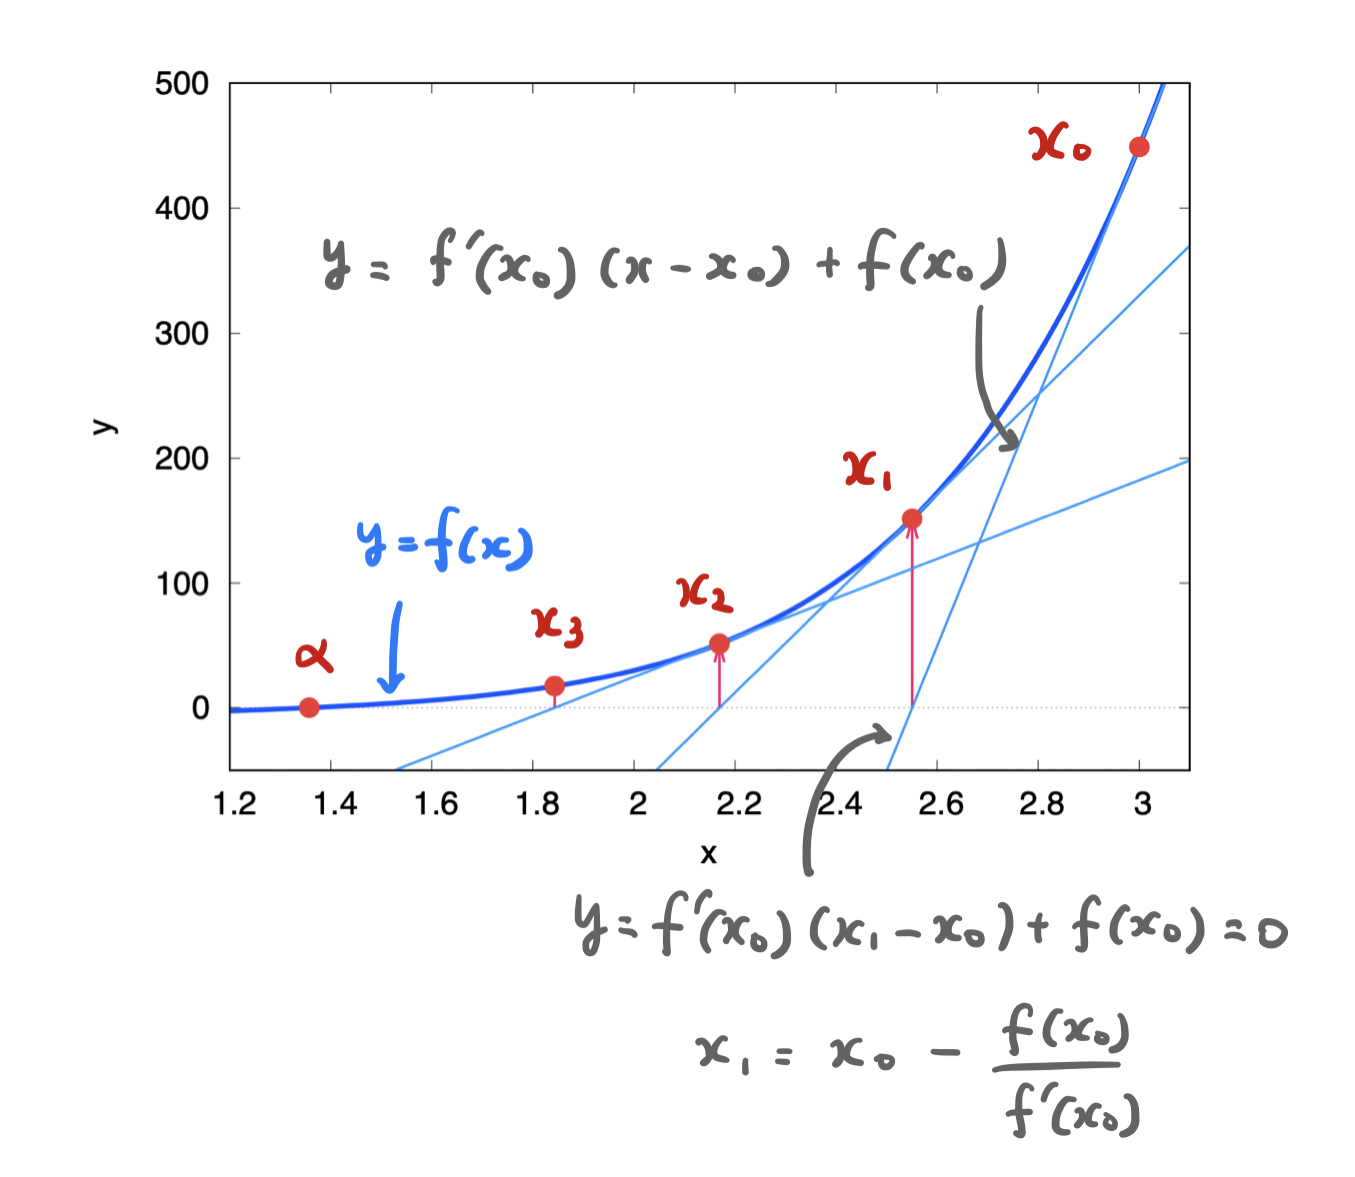
\includegraphics[width=0.94\textwidth]{fig04-1_newtons_method_proof.jpeg}
	\end{center}
\end{figure}
\end{column}
\end{columns}
\end{frame}
%%%%%%%%%%%%%%%%%%%%%%%%%%%%%%%%
\begin{frame}
\frametitle{\large [解説] ニュートン法の解析的導出}
\begin{itemize}
    \setlength{\itemsep}{0.3cm}
    \myfontsetting{15pt}{17pt}{
    \item $f(x)$ の求めたい根の真値を $\alpha$ とする。$x_k \approx \alpha$ のとき $f(x)$ の $x=x_k$ でのテイラーの定理を考えると $f(x) = f(x_k) +f^\prime(x_k)(x-x_k)+\frac{f^{\prime\prime}(\xi_k)}{2!}(x-x_k)^2$ となる。
    \item $x=x_{k+1}$ とし、 $f(x_{k+1})<<f(x_k)$, $\frac{f^{\prime\prime}(\xi_k)}{2!}(x_{k+1}-x_k)^2<<f(x_k)$ が成り立つと仮定して左辺と右辺第3項を0と置くと $0=f(x_k)+f^\prime(x_k)(x_{k+1}-x_k)$ より   $x_{k+1}=x_k - \frac{f(x_k)}{f^\prime(x_k)}$となる。
    }
\end{itemize}
\end{frame}
%%%%%%%%%%%%%%%%%%%%%%%%%%%%%%%%
\begin{frame}
\frametitle{\large [解説] 収束の速さ}
\begin{block}{{\bf 収束の次数} {\small (Order of convergence for sequences)}}
\myfontsetting{18pt}{20pt}{$x_k$ が $\alpha$ に収束し $\lim_{k\to \infty}\frac{\alpha - x_{k+1}}{(\alpha - x_k ) ^p} = A$ を満たすような非零で有限な定数 $A$ を持つとき、$p$ を $x_k$ の{\bf 収束の次数}という。}
\end{block}
\begin{itemize}
    \setlength{\itemsep}{0.5cm}
    \item \myfontsetting{18pt}{20pt}{ニュートン法では $p=2$ であり、{\bf 2次収束}と呼ぶ}
\end{itemize}
\end{frame}
%%%%%%%%%%%%%%%%%%%%%%%%%%%%%%%%
\begin{frame}
\frametitle{\large [解説] 2次収束の証明}
\begin{block}{{\bf ニュートンの誤差公式} {\small (Newton error formula)}}
\myfontsetting{15pt}{18pt}{
ある区間 $I\subset \mathbb{R}$ で $f\in C^2(I)$ が根 $\alpha$ を持ち、$x_k\in I$ に対して $x_{k+1} = x_k - \frac{f(x_k)}{f^\prime(x_k)}$ $(f^\prime(x_k)\neq 0)$ という数列を考える。このとき $\alpha$ と $x_k$ の間に $\xi_k$ が存在して
$\alpha - x_{k+1} = -\frac{1}{2}(\alpha - x_k)^2 \frac{f^{\prime\prime}(\xi_k)}{f^\prime(x_k)}$
が成り立つ。
}
\end{block}
\begin{itemize}
    \setlength{\itemsep}{0.5cm}
    \item \myfontsetting{15pt}{18pt}{ここから $\lim_{k\to \infty}\frac{\alpha - x_{k+1}}{(\alpha - x_k ) ^2} = -\frac{f^{\prime\prime}(\alpha)}{2f^\prime(\alpha)}$ ({\bf 2次収束}) が示せる。}
\end{itemize}
\end{frame}
%%%%%%%%%%%%%%%%%%%%%%%%%%%%%%%%
\begin{frame}
%%%%% PASTE_START_TAG B %%%%%
%\noindent{\bf I\hspace{-.1em}V-B.}
\frametitle{[問題] I\hspace{-.1em}V-B}
\myfontsetting{16pt}{18pt}{
ニュートン法により
}
\myfontsetting{14pt}{16pt}{
$f(x)=2-e^{x}$
}
\myfontsetting{16pt}{18pt}{
の根を求めるプログラムを初期値を $x=1$ として作成し、根の真値を有効数字10進16桁まで示した
}
\myfontsetting{14pt}{16pt}{
$\alpha=0.6931471805599453$
}
\myfontsetting{16pt}{18pt}{
と比べて絶対誤差が $10^{-8}$ 以下となる最低の反復回数 $n$ を求めよ。
また $n$ 回反復した時の根の近似値と絶対誤差も求めよ。近似値は有効数字10進11桁以降を切り捨てて求め、絶対誤差は有効数字10進4桁以降を切り捨ててよ。
}\\
\myfontsetting{12pt}{14pt}{
作成したプログラムも提出すること。プログラミング言語は問わない。
}
%%%%% PASTE_END_TAG B %%%%%
\end{frame}
%%%%%%%%%%%%%%%%%%%%%%%%%%%%%%%%
\end{document}
